\chapter{Experiments}

We now evaluate our proposed methods empirically in various settings.
Through the experiments, we aim to answer the following questions:

\begin{itemize}
	\item How does the addition of the NeuRD-fix, Extragradient updates, Optimism
	      affect the convergence rate of these algorithms in solving for QREs, and Nash equilibrium?
	\item What is the last-iterate vs average-iterate convergence behavior of these algorithms in the presence of these modifications?
	\item Do these performance improvements scale well with the size of the game?
\end{itemize}

\section{Experimental Domains}
In answering the above questions, we consider both tabular and function approximation settings.
For the tabular experiments we evaluate the performance of these algorithms for convergence to QRE
and Nash equilibrium.
methods using the following environments - Perturbed
RPS.

For the function approximation setting, we evaluate the algorithms on Kuhn Poker, Abrupt Dark Hex,
and Phantom Tic-tac-toe.
Kuhn Poker is a smaller extensive form game that allows for more introspection and accurate
measurement of performance.
Whereas, Abrupt Dark Hex, and Phantom TTT are large games that test the stability of these
modifications in settings with a large state-space.

\section{Evaluation Methods}

Typically, to measure the convergence rate of an algorithm we can use either a a measure of
distance from an equilibrium if the equilibrium point is known or, a measure of exploitability as
an indication of the policies reaching the equilibrium.

For tabular settings since the equilibrium solutions are known, we use both exact exploitability
and KL-divergence to the equilibrium to evaluate the algorithms.
For PerturbedRPS, we use the QRE solutions computed through Gambit and, we also derive the unique
Nash Equilibrium (please refer to \ref{sec:rpsne} in the appendix for the derivation) for
PerturbedRPS.

-Define exact exploitability

For the function approximation settings we use the above metrics for the smaller games Kuhn Poker,
and 2x2 Dark Hex which also have equilibrium solutions computed through Gambit.
For the larger games, since exact exploitability computation is not possible and we do not know the
equilibrium solution, we use an approximate measure of exploitability by using a DQN to approximate
the best response computation similar to~\cite{sokotaUnified2023}.

\section{Results}

\subsection{Tabular Experiments}
Below, we give an overview of Last, and Average iterate convergences of 3 different algorithms -
MMD, MDPO, SPG, and their variants obtained by applying combinations of the modified updates.
We give the convergence results for the more interesting behaviors observed, a more exhaustive list
of all combinations and their convergence behaviors can be found in the appendix.

% \begin{noindent}
\begin{table}
	\centering
	\begin{tabular}{|c|c|c|c|c|c|c|c|c|c|c|}
		\hline
		& \multicolumn{2}{c|}{Nash} & \multicolumn{2}{c|}{QRE ($\alpha$=0.5)}              \\
		\cline{2-5}
		Algorithm         		& Avg & Last & Avg & Last \\
		 \toprule 
		\hline MMD (cf)			& y & y & y & y \\ 
		\hline FMMD (bf)		& y & y & y & y \\
		\hline FMMD-N			& y & x & x & x \\
		\hline FMMD-EG			& y & y & y & y \\
		\hline FMMD-N-EG		& y & y & x & x \\
		\hline FMMD-N-OPT		& y & x & x & x \\
		\hline MDPO				& x & x & - & - \\
		\hline MDPO-N			& x & x & - & - \\
		\hline MDPO-EG			& y & y & - & - \\
		\hline MDPO-N-EG		& y & y & - & - \\
		\hline MDPO-EG-OPT		& y & y & - & - \\
		\hline MDPO-N-EG-OPT	& y & y & - & - \\
		\hline

	\end{tabular} \caption{Convergence in Perturbed RPS}
	\label{tab:tabular}
\end{table}
% \end{noindent}

Apart from the final convergence results, we also make a few observations regarding the speed of
convergence for these variants.
From \ref{fig:divplots}, we note the following

\begin{figure}[H]
	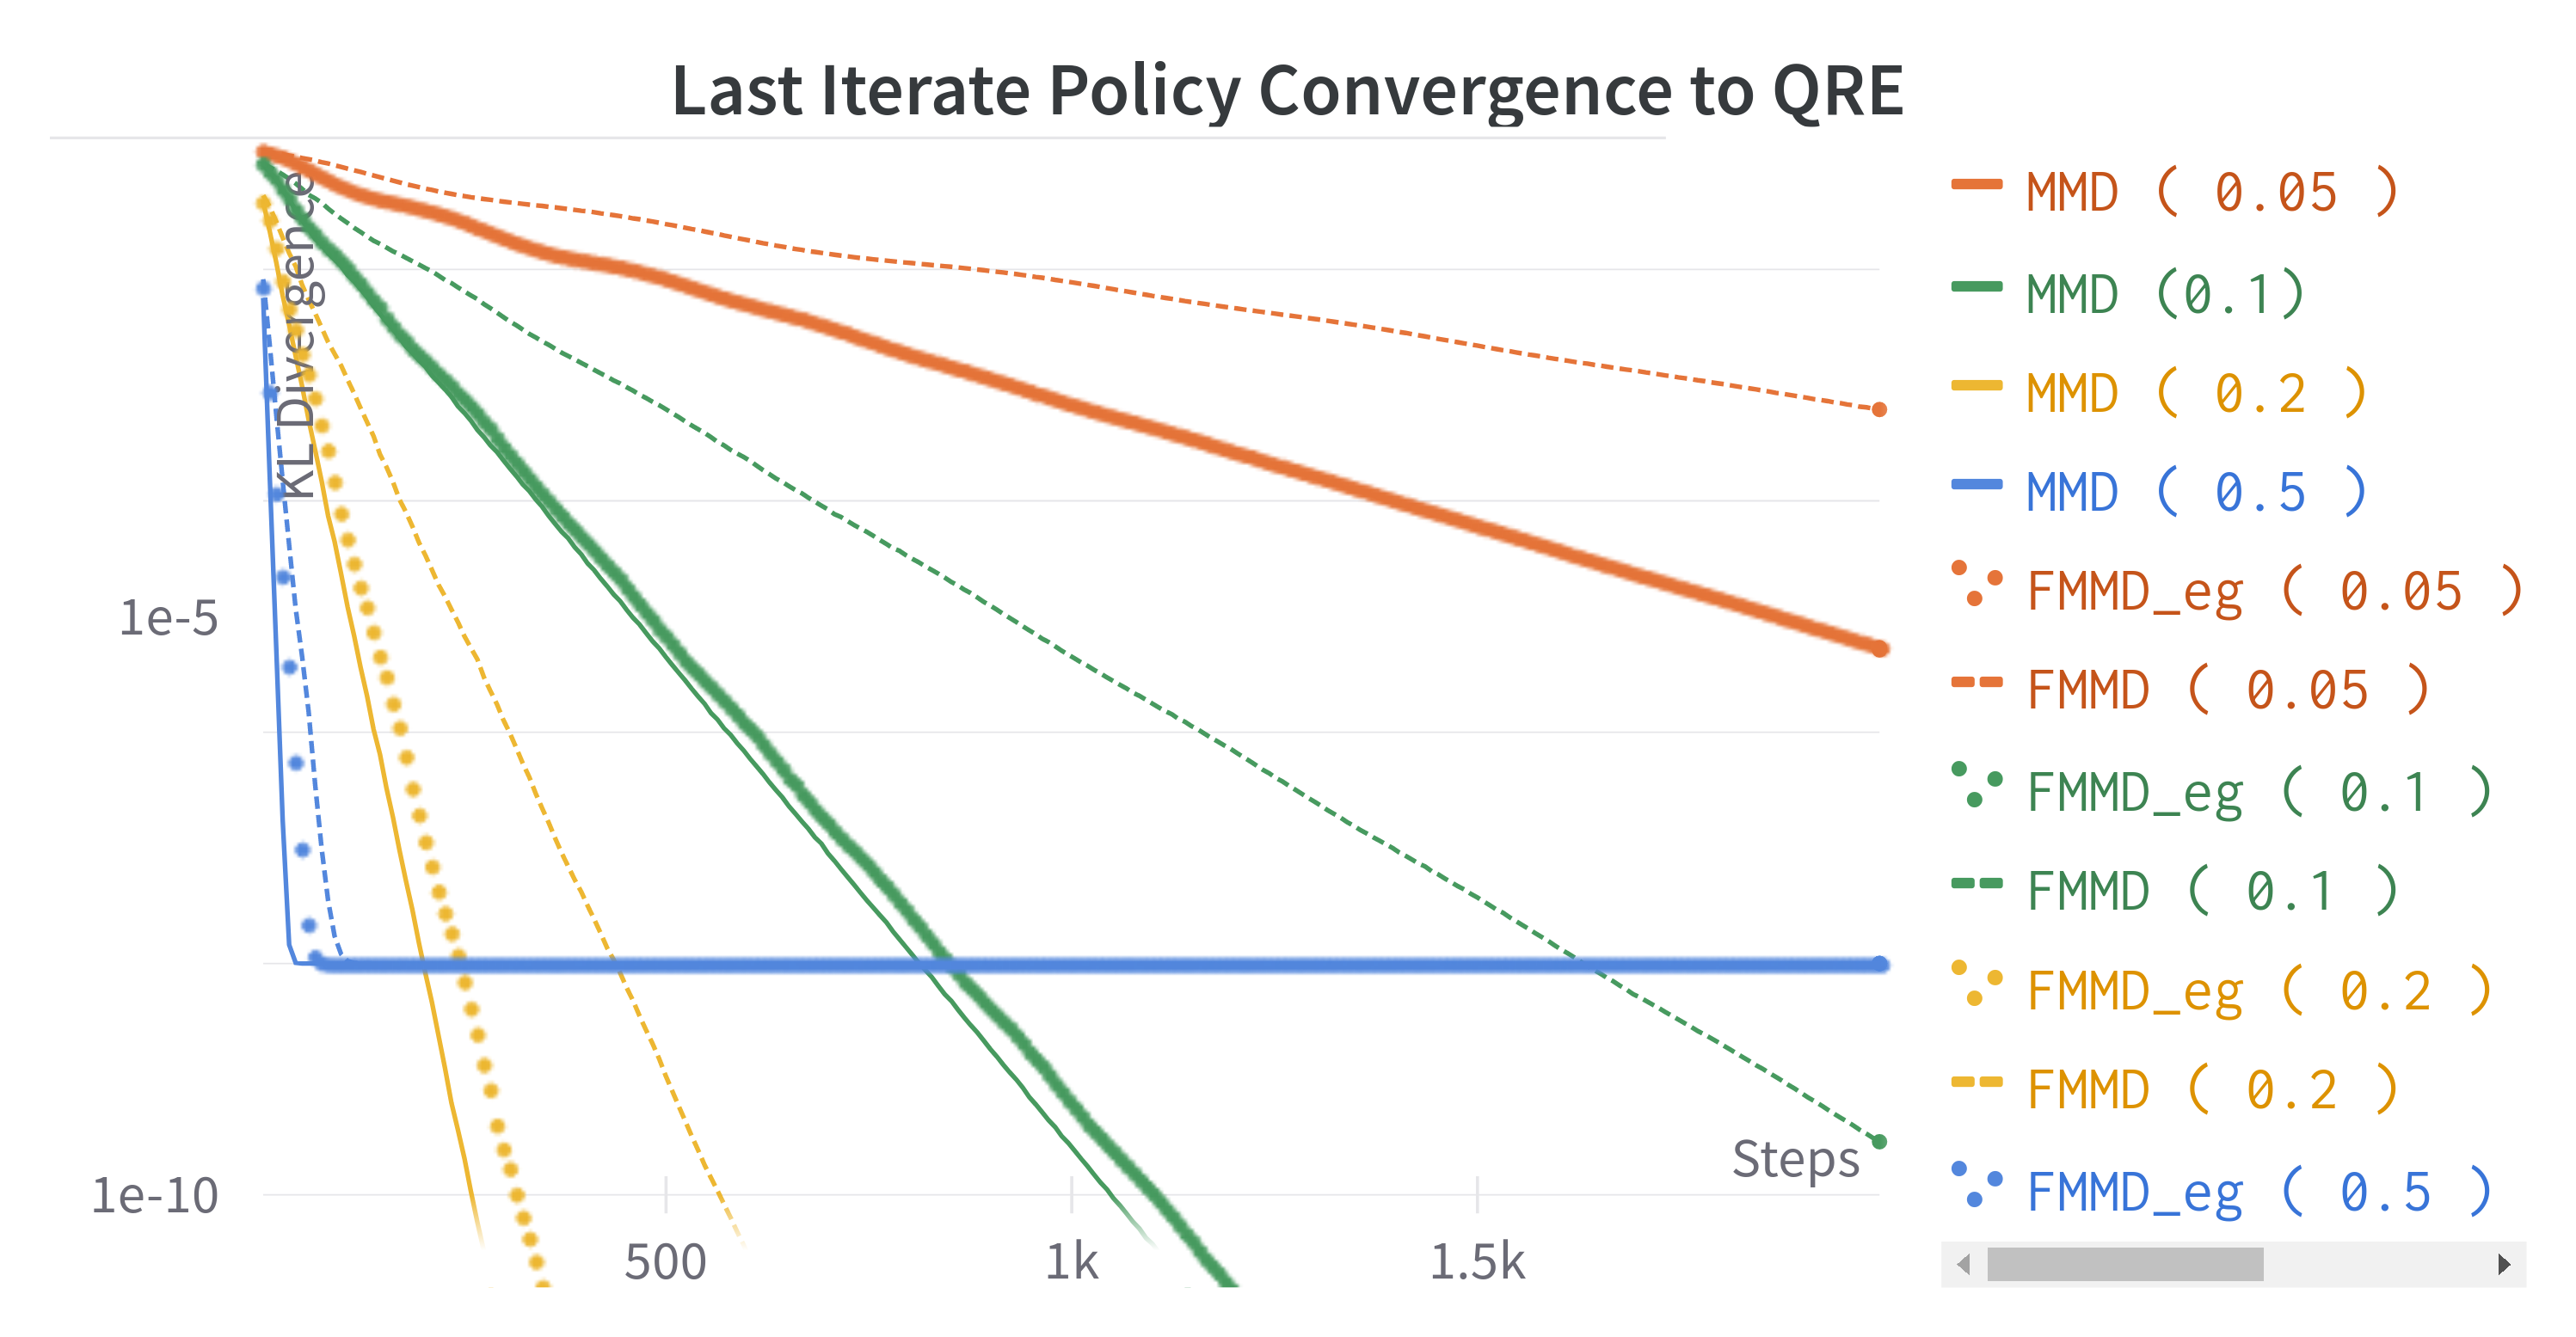
\includegraphics[width=15cm]{FIG/MMD_QRE.png}
\end{figure}

\begin{figure}[H]
	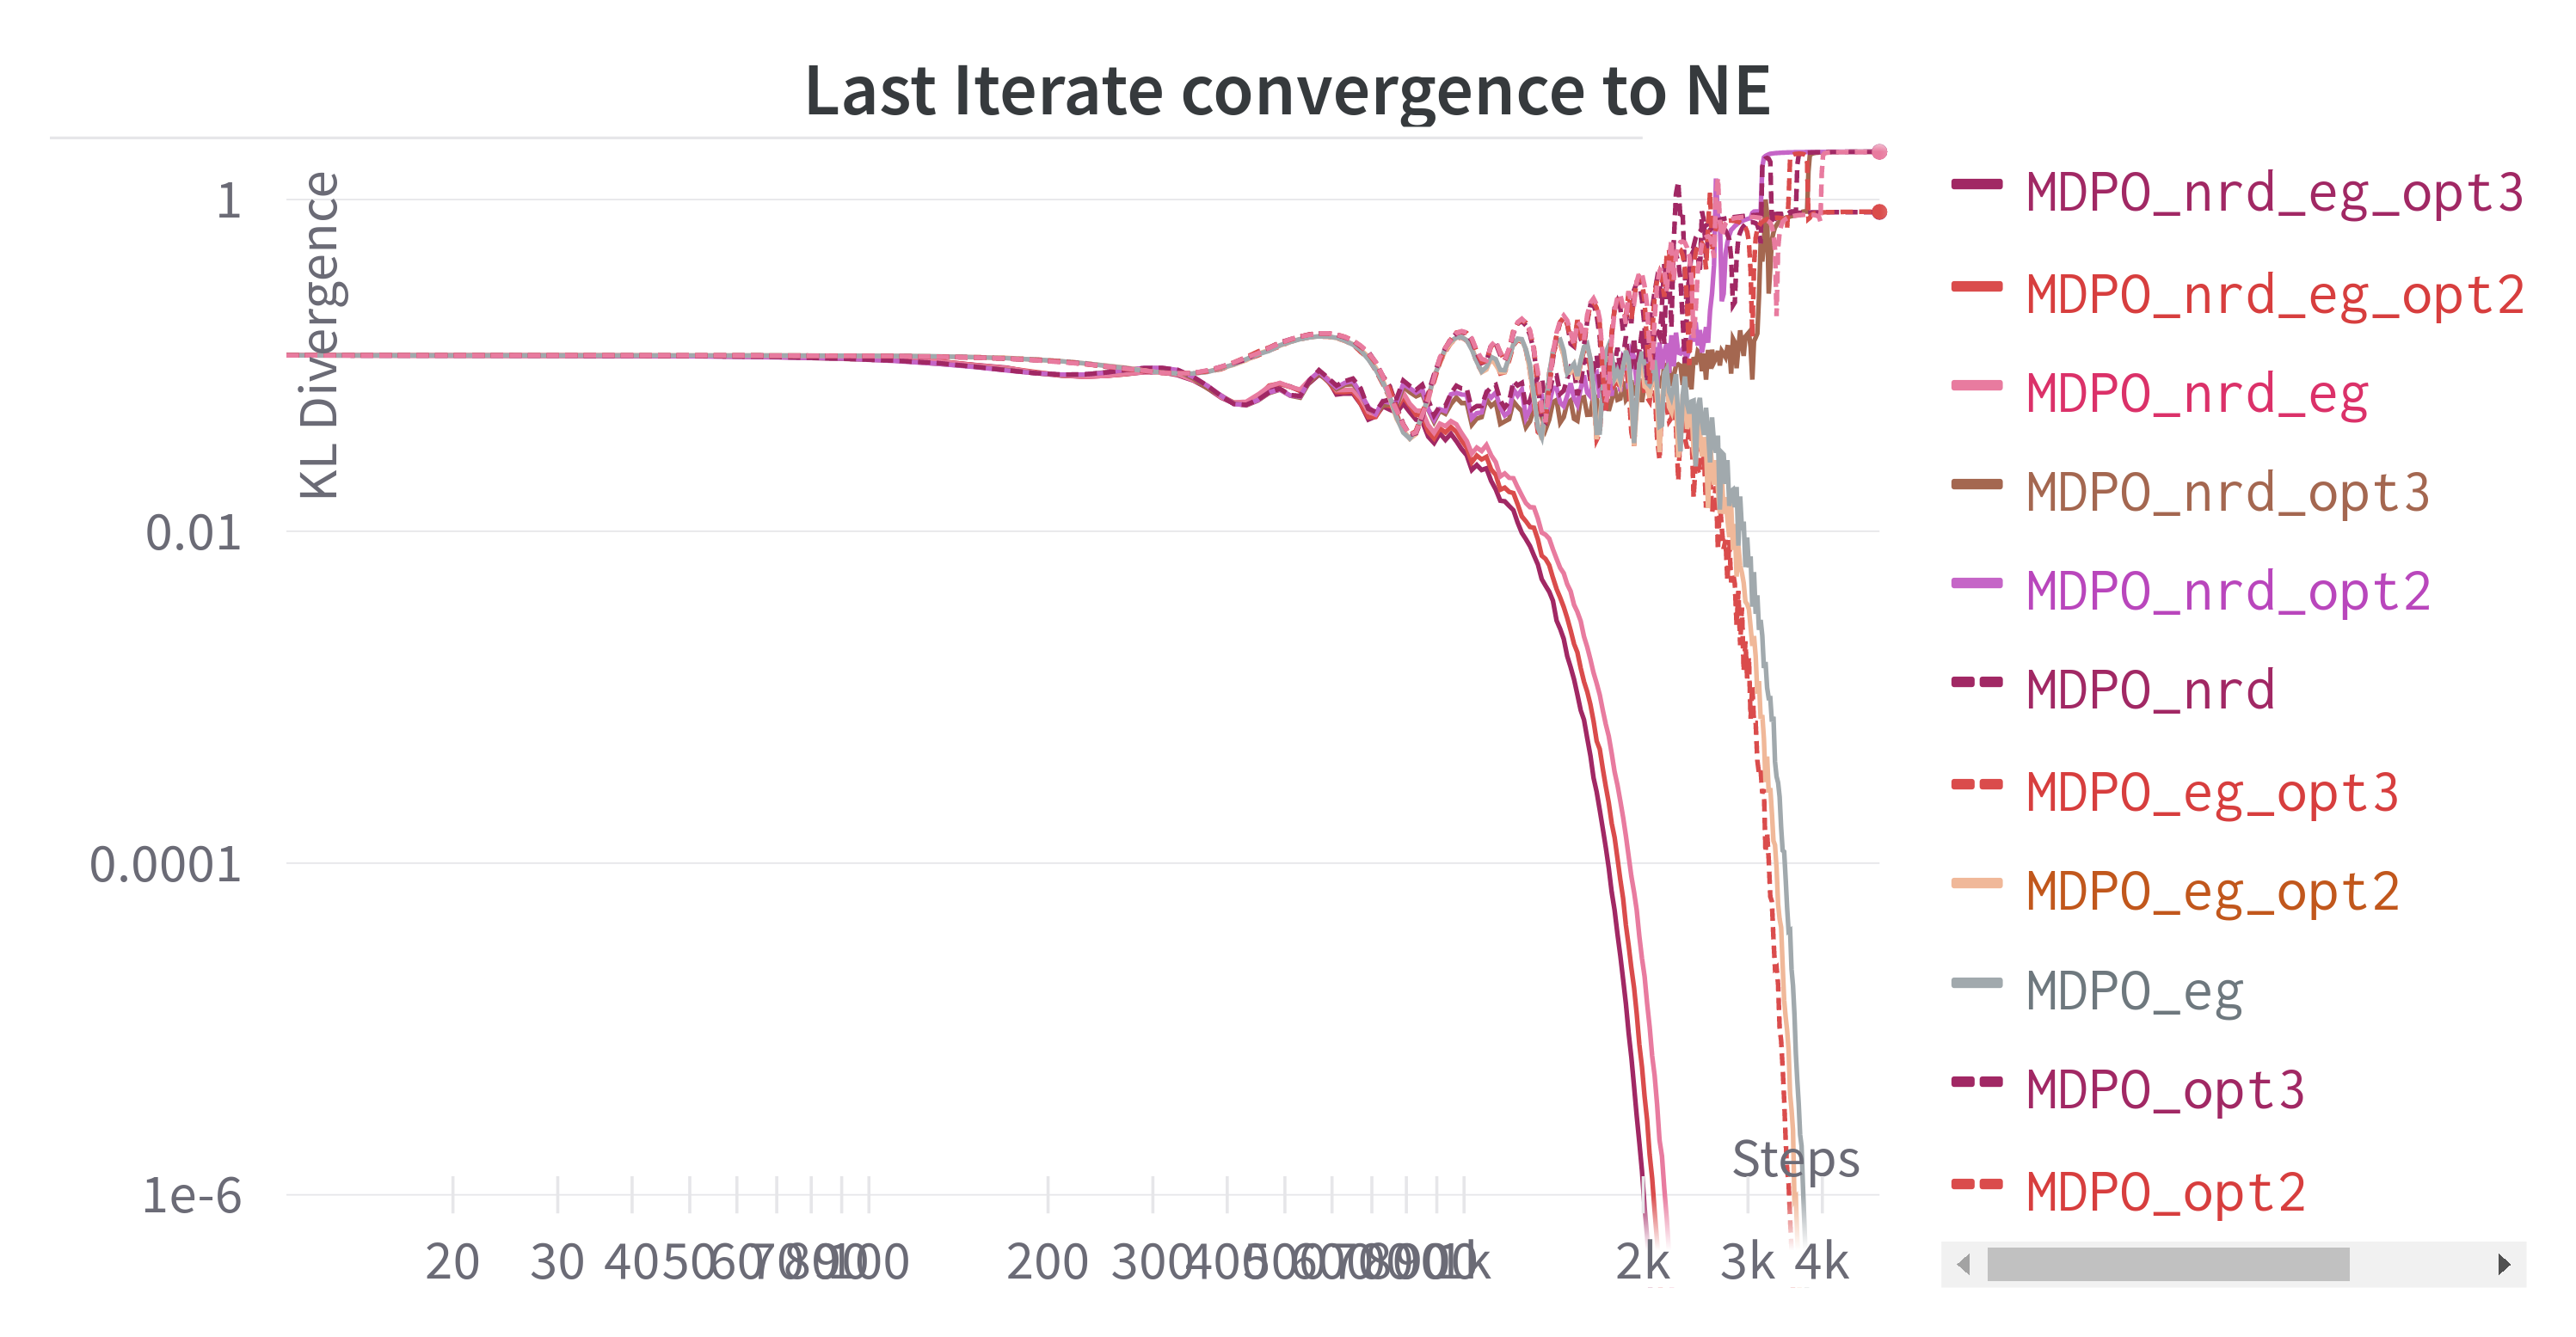
\includegraphics[width=15cm]{FIG/MDPO_NE.png}
\end{figure}

\begin{figure}[H]
	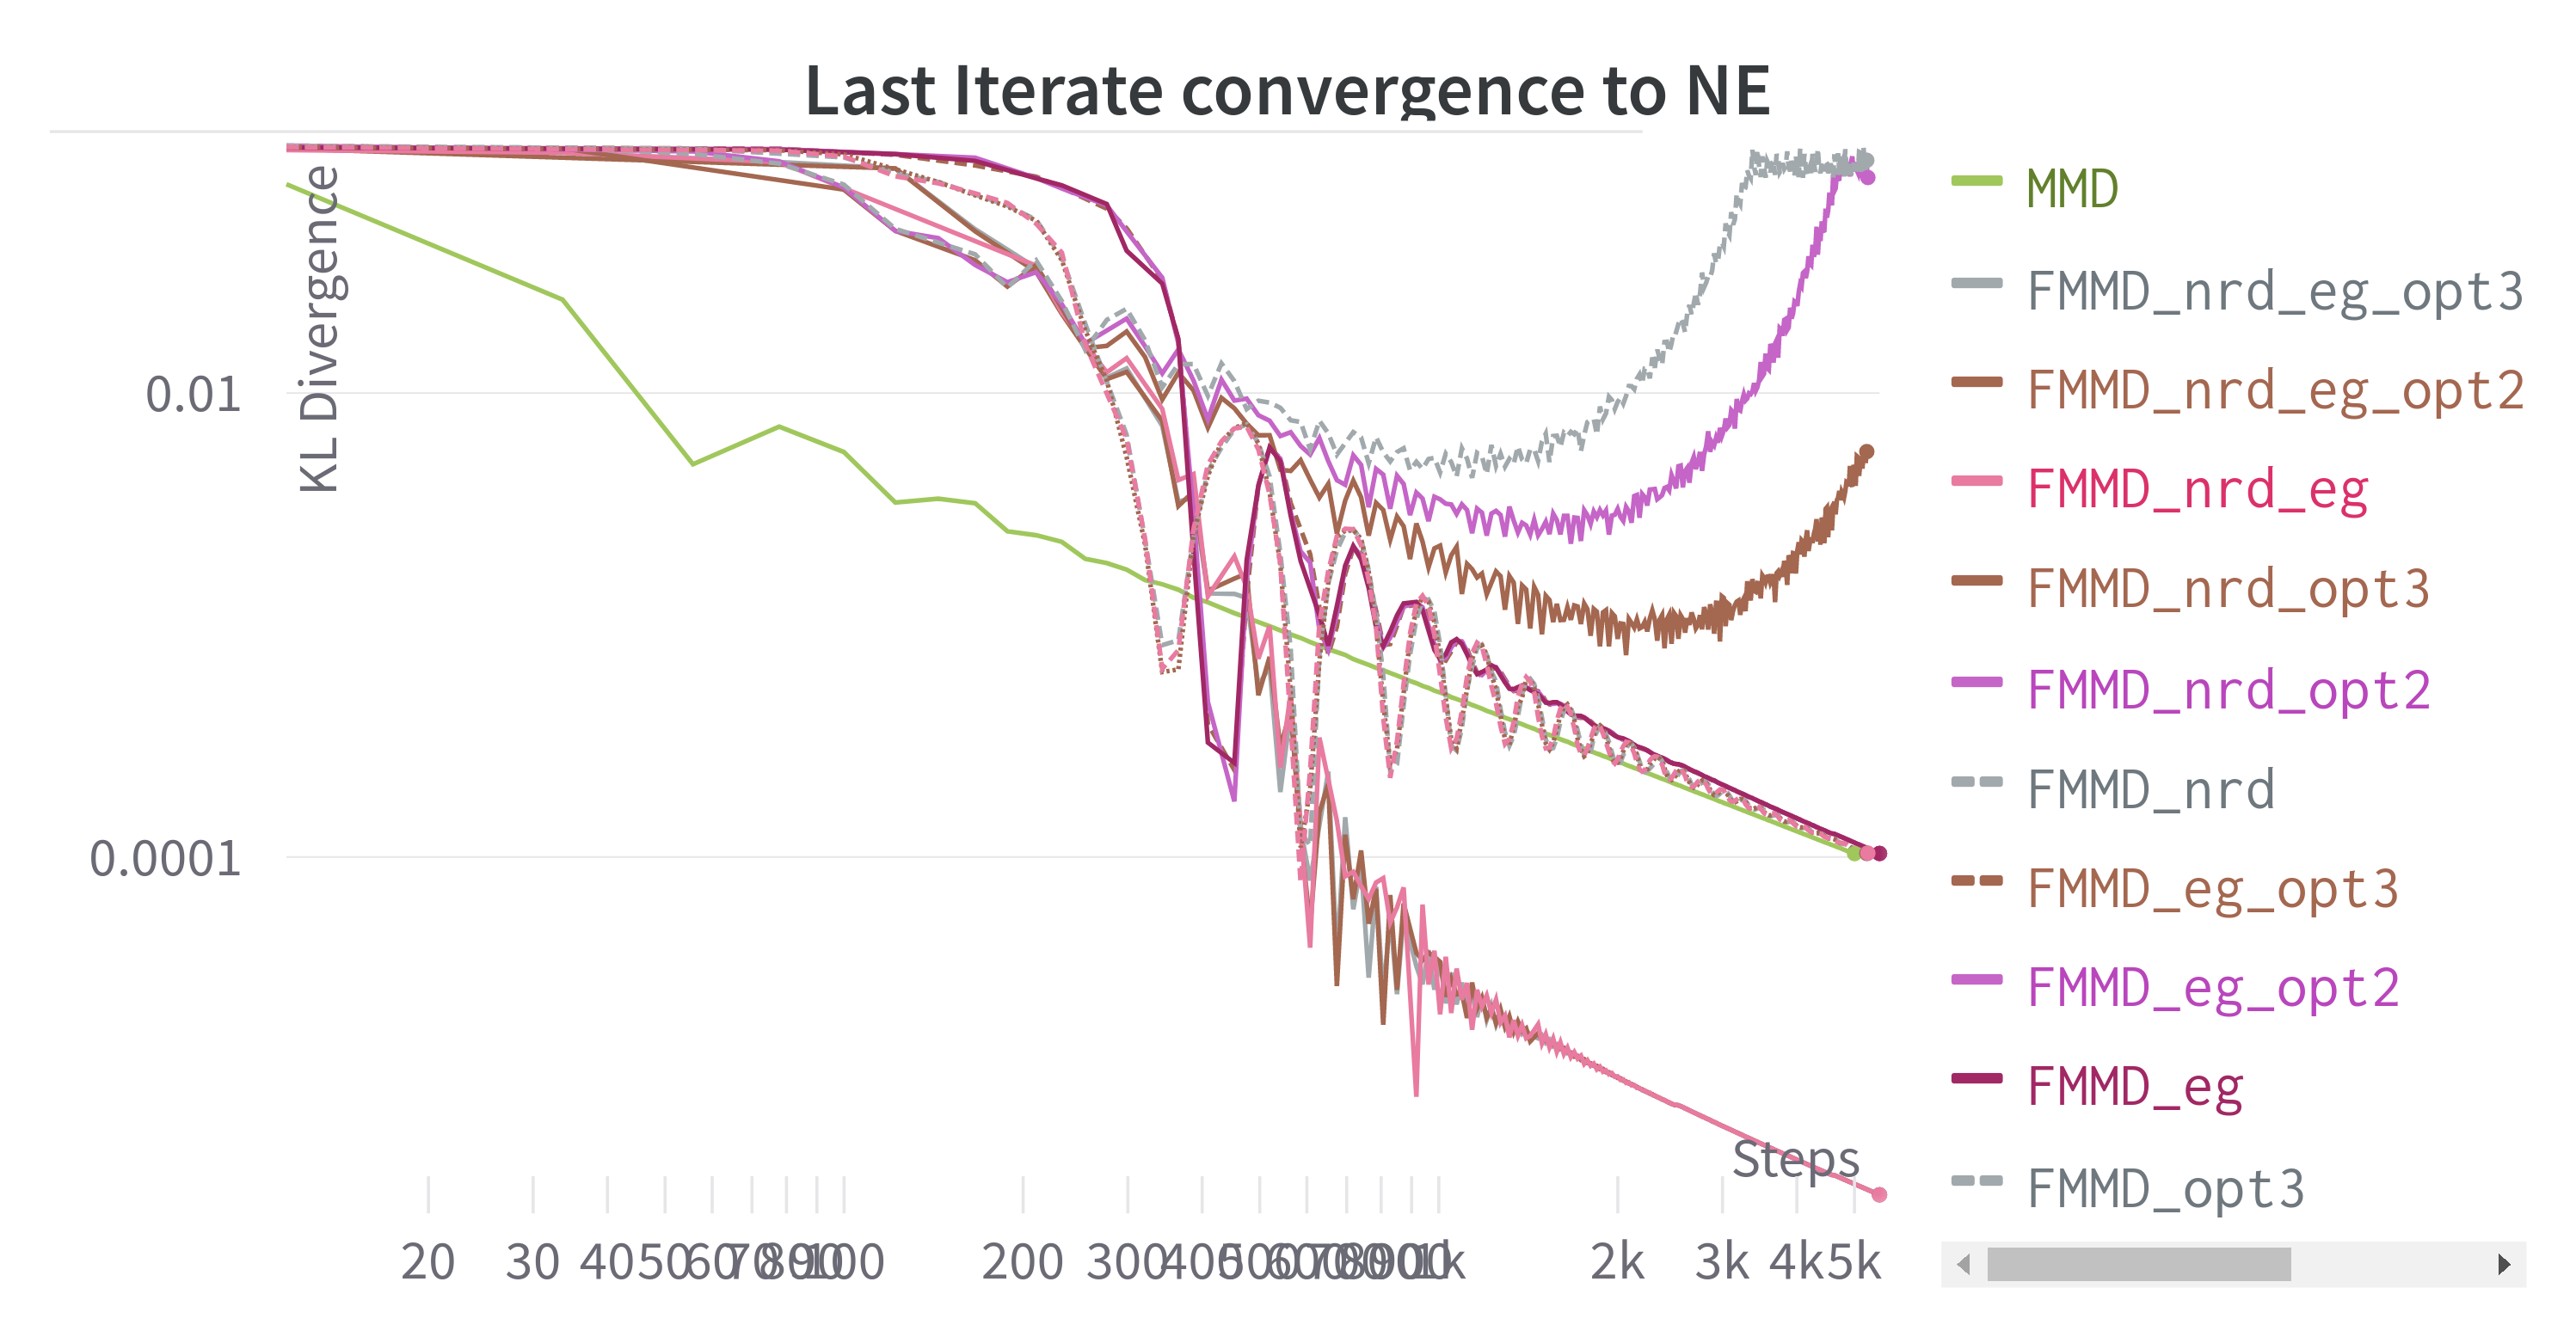
\includegraphics[width=15cm]{FIG/MMD_NE.png}
\end{figure}

\begin{itemize}
	\item{MDPO with extragradient updates have superlinear last iterate convergence to Nash
	            equilibrium.
	      }
	\item{MMD with NeuRD fix and extragradient }
\end{itemize}

\subsection{Neural Experiments}

Based on the observations from the Tabular NFG experiments, we evaluate the most promising
combinations of these algorithms in the function approximation setting.
As discussed in~\cite{sokotaUnified2023}, behavioral form MMD can be implemented as a reinforcement
learning algorithm with minor changes to PPO due to its similarity.
We implemented MMD, in a similar way as described in~\cite{sokotaUnified2023} by modifying the PPO
implementation in RLLib~\cite{liangRLlib2018}.
We also use RLLib's OpenSpiel adapter with some modifications to use information states as inputs
as opposed to observations.
We train these reinforcement learning agents in self-play for the environments mentioned above.

- Implementation details (RLLib, PPO modifications, GAE)
- Neural network architecture, hyperparameters

